\chapter{Introduction}


\section{Introduction to the Ubiquitin 26S Proteasome System}
Selective proteolysis in plants plays a critical role in both regulating growth and development, and maintaining cellular homeostasis \citep{nelson14, smalle04, vierstra93, vierstra09}.  One of the principle pathways for protein degradation in plants and other eukaryotes is the ubiquitin-26S proteasome system (UPS), which involves the attachment of polyubiquitin chains to target proteins followed by their recognition and degradation by the 26S proteasome, an exquisitely designed proteolytic machine \citep{bhattacharyya14, finley09, vierstra09}.  The UPS is highly conserved across all eukaryotes; it was first elucidated by elegant work in rabbit reticulocyte lysates \citep{ciechanover80, ciechanover80-frAQB, etlinger77, hershko80, wilkinson80}, and was subsequently identified in other animals, yeast and higher plants \citep{ciechanover84, finley84, finley87, glotzer91, hochstrasser91, shanklin87}.  Ubiquitin conjugation to target proteins is accomplished through a highly polymorphic, ATP-dependent cascade involving the sequential action of three enzyme classes, termed the E1 ubiquitin-activating enzymes, E2 ubiquitin-conjugating enzymes, and E3 ubiquitin-protein ligases (\ref{fig:UPScycle} \citep{berndsen14, smalle04, vierstra09}.  Selectivity in ubiquitylation is driven by the E3 family, which has dramatically expanded during plant evolution to include well over a thousand variants in \textit{Arabidopsis thaliana} and other plant species \citep{hua13, hua11}.  Through this myriad of E3s combined with the 26S proteasome, plants precisely control the levels of many key intracellular regulators that impact most, if not all, aspects of plant biology \citep{kim13, vierstra09}.
\begin{sidewaysfigure}[p]
	\centering
	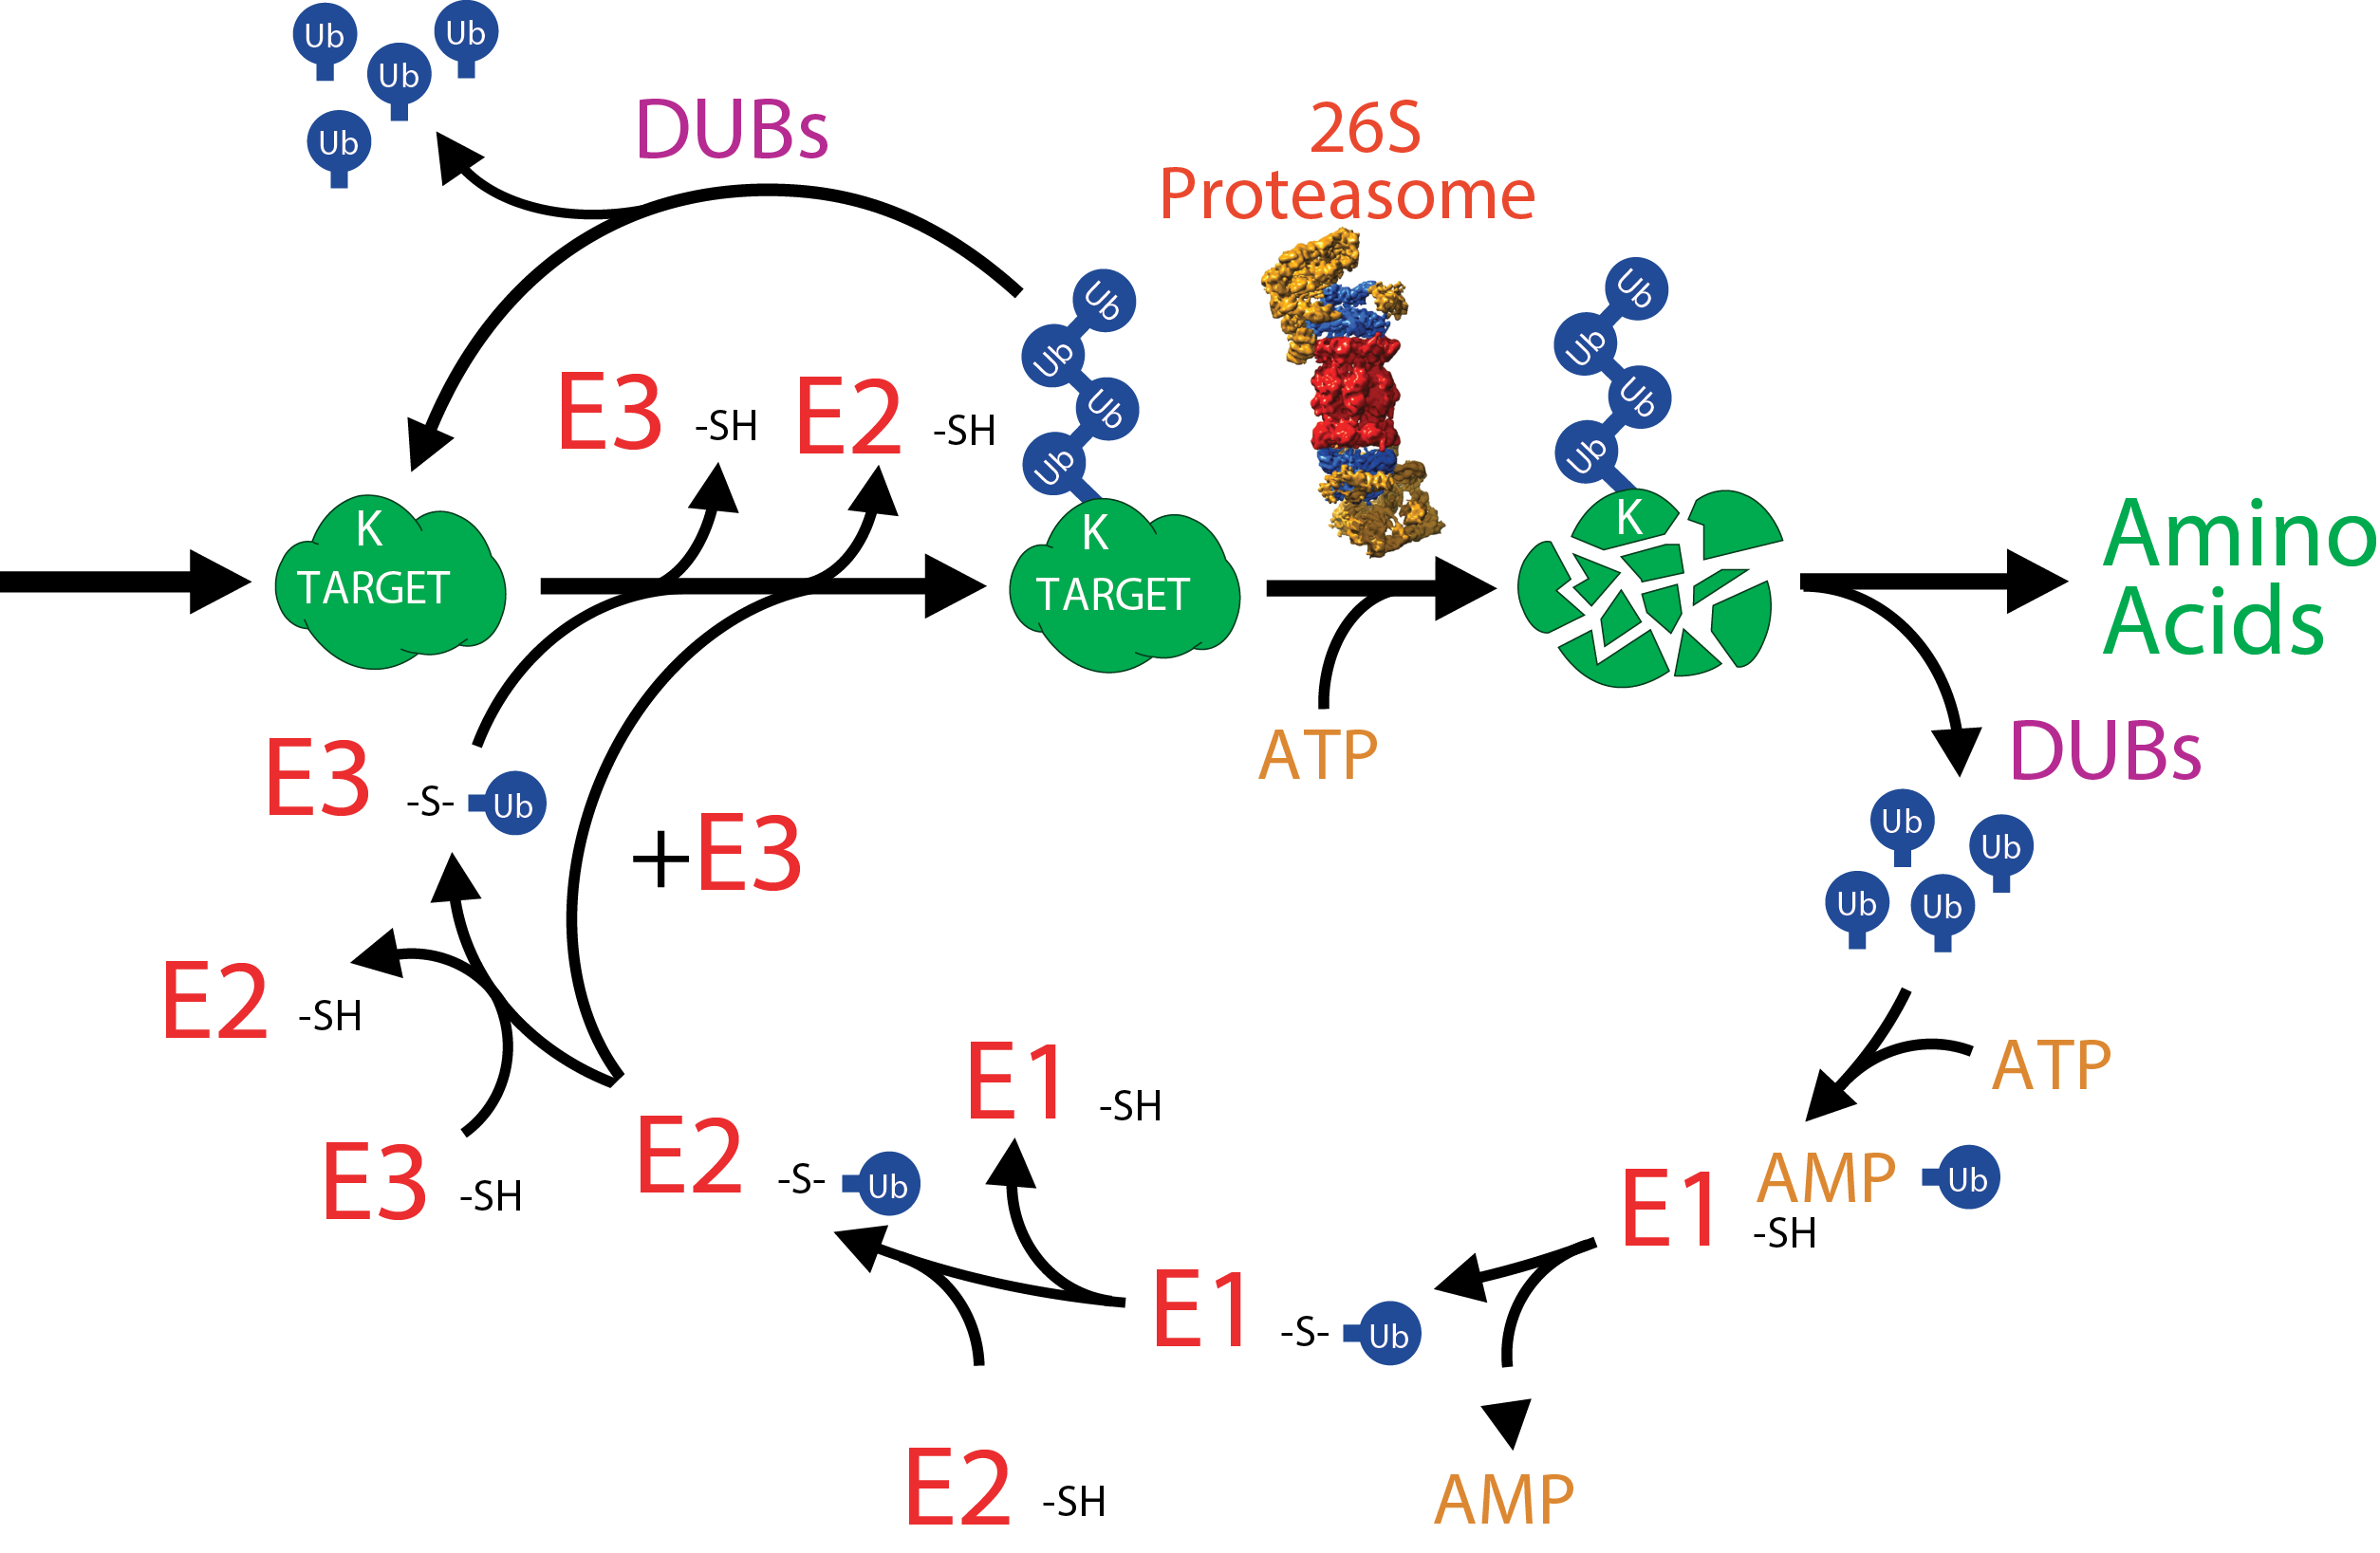
\includegraphics[width=\columnwidth]{intro/upscycle.png}
	\mycaption{The Ubiquitin 26S Proteasome System}{
	Target proteins are covalently modified by ubiquitin an ATP-dependent E1 activating, E2 conjugating, E3 ligase enzymatic cascade. Once a target protein becomes polyubiquitylated, typically with a K48 linkage, it is efficiently recognized and subsequently degraded by the 26S proteasome.  Ubiquitin is released from the target protein by various de-ubiquitylating enzymes (DUBs) and can then enter the cycle again to covalently modify other substrates. 
	}
	\label{fig:UPScycle}
\end{sidewaysfigure}
\section{The 26S Proteasome}
	The 26S proteasome is a 2.5 MDa particle located in the cytosol and nucleus of eukaryotic cells.  It is composed of two functionally distinct sub-complexes; the 20S core protease (CP) that houses the proteolytic active sites, and the 19S regulatory particle (RP) that recognizes appropriate substrates (Figures \ref{fig:proteasomefunc} A and B; \citep{bhattacharyya14, finley09, lander12, lasker12, unverdorben14}).
\begin{figure}[p]
	\centering
	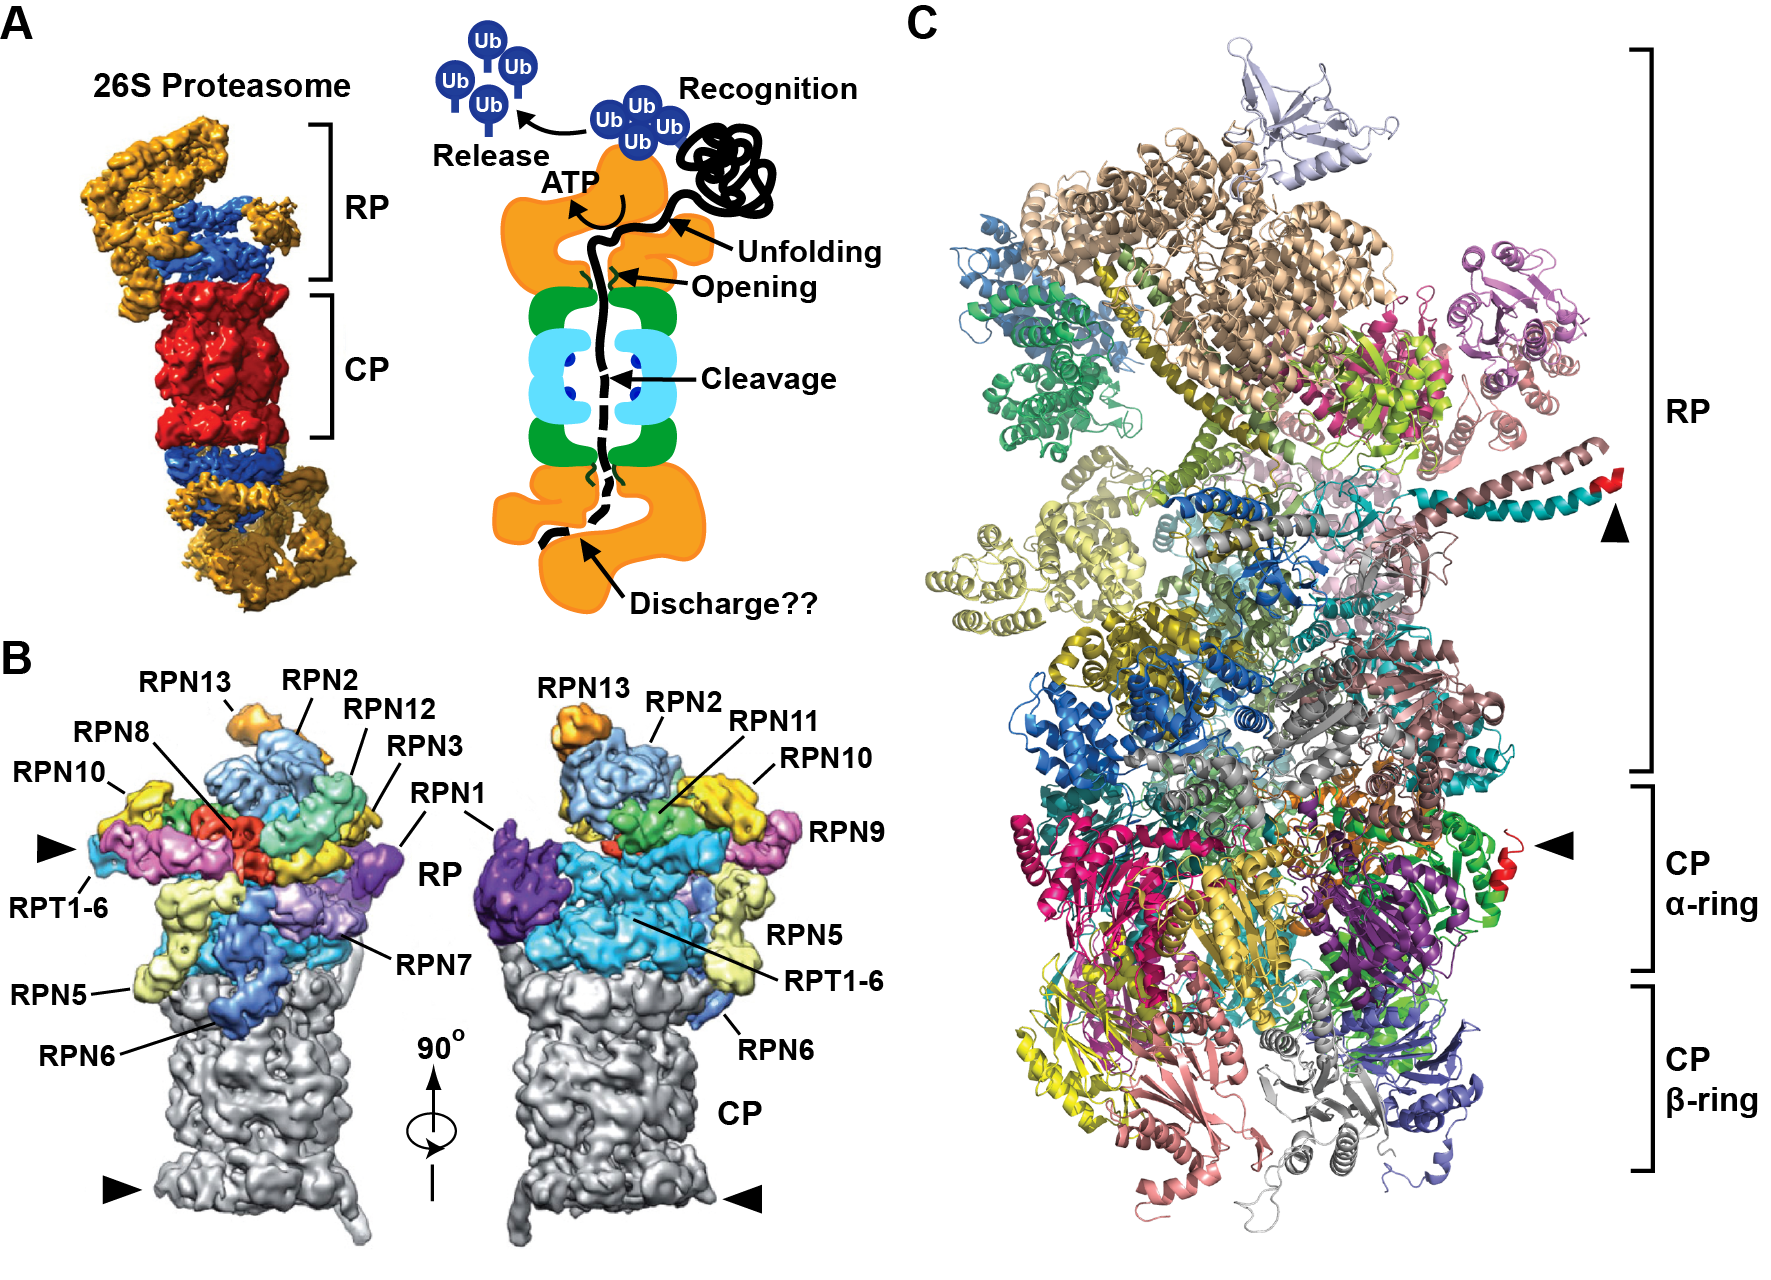
\includegraphics[width=\columnwidth]{intro/figure1.png}
	\mycaption{Structure of the 26S proteasome}{
		\textbf{(A)} Schematic representation of the 26S proteasome, with a 3-D structure as determined by electron microscopy (EM) shown on the left, and a cartoon representation of the holoprotease shown on the right.  Within the EM structure, the CP is shown in red, the RP base is shown in blue, and the RP lid is shown in yellow.  Specific functions within the CP and RP are shown on the right.  The EM structure is modified from reference \citep{lasker12} \textbf{(B)} A detailed view of the subunit architecture of the 26S proteasome RP.  The CP is shown in grey, the RPT ring is shown in blue, and all additional RPN subunits are shown in different colors, with their identity labelled.  The positions of the FLAG tags on PAG1 and RPT4 are indicated by red arrowheads.  These structures are modified from reference \citep{lander12}.  \textbf{(C)} A structural model of the 26S proteasome from yeast at sub-atomic resolution modified from PDB ID 4CR2 \citep{beck12}.  The RP subunits, as well as the CP $\alpha$ and $\beta$ rings are shown.  Highlighted in red, and indicated by black arrowheads, are the positions where FLAG affinity tags have been successfully used to enrich for Arabidopsis 26S proteasomes. The affinity purification of the RP developed as part of the dissertation (Chapter 3) exploits the tag shown in the regulatory particle.
	}
	\label{fig:proteasomefunc}
\end{figure}
	 The CP has a barrel shape generated by four stacked hetero-heptameric rings, which contain seven $\alpha$-subunits or seven $\beta$-subunits (termed PAA-PAG and PBA-PBG, respectively, in \textit{Arabidopsis}) in an $\alpha$1-7/$\beta$1-7/$\beta$1-7/$\alpha$1-7 configuration.  Upon assembly, a central chamber is formed at the $\beta$-ring interface that houses six peptidase catalytic sites provided by the $\beta$1 (PBA), $\beta$2 (PBB), and $\beta$5 (PBE) subunits \citep{arendt97, heinemeyer97}.  The active sites involve a catalytic triad, one residue of which is an N-terminal threonine that becomes exposed during CP assembly.  Collectively these peptidases can cleave a broad range of protein sequences with peptidylglutamyl-peptide hydrolyzing (PGPH) ($\beta$1), trypsin-like ($\beta$2), and chymotryptic-like ($\beta$5) activities  \citep{arendt97, groll99}.  The $\alpha$-rings create two antechambers with narrow opposing axial pores that are gated by extensions at the N-terminus of several subunits \citep{groll00, ruschak10}.  Through this distinctive architecture, the CP acts as a self-compartmentalized protease that will only degrade polypeptides that are deliberately recognized, unfolded, and imported into the $\beta$-ring chamber. 
	The CP is capped at one or both ends by the RP, which sits on top of the axial pores.  The RP provides activities for recognition of ubiquitylated proteins, substrate unfolding and import, and release of the ubiquitin moieties before substrate degradation.  Its binding to the CP is stabilized by ATP, which is thus a necessary ingredient for purifying intact 26S proteasomes.  The RP itself consists of two sub-complexes; the base, which contains a hexameric ring of AAA-ATPases (RPT1-6) plus two non-ATPase subunits, RPN1 and RPN2; and the lid, which is composed of an additional 11 non-ATPase subunits, RPN3, RPN5-13 and DSS1/SEM1 (Figures \ref{fig:proteasomefunc} B and C; \citep{bhattacharyya14, book10, finley09, glickman98-c8Wsa, russell13}.  This lid/base demarcation was first revealed by the absence of lid subunits in proteasomes isolated from a $\Delta$rpn10 yeast deletion strain, and it was hence thought that RPN10 helps enforce binding of the lid to the base \citep{glickman98}.  However, more recent structural studies have demonstrated that RPN10 has a more indirect stabilizing role via its interaction with RPN9 \citep{lander12}.  The ring of RPT subunits in the base promotes substrate unfolding through ATP hydrolysis, and gates the $\alpha$-ring axial pores through repositioning of the CP $\alpha$-subunit extensions \citep{köhler01, rabl08, smith05}.  The N-terminal regions from proximal RPT pairs intertwine to create three spokes onto which most RPN subunits are scaffolded (Figure \ref{fig:proteasomefunc} C; \citep{beck12}).  The RPN6 subunit acts as a molecular clamp to tether the RP onto the CP (Figure \ref{fig:proteasomefunc} B; \citep{pathare12}. 


\section{Proteasome Purification Strategies}
	Even before the realization that the 26S proteasome is a protease, sub-particles of the complexes were described.  The first reports of proteasomes used avian erythroblast preparations enriched by differential ultracentrifugation followed by fractionation through a sucrose gradient \citep{schmid84}.  These 20S fractions isolated in the absence of added ATP were found to inhibit mRNA translation in a cell-free system, leading to early proposals that the identified complex repressed gene expression through a cryptic ribonuclease activity.  This lead to the particle initially being named the ``prosome'' \citep{kremp86, schmid84}.  Subsequent analyses of these preparations by SDS-PAGE and electron microscopy revealed the signature ladder of $\alpha$- and $\beta$-subunits at 20-35 kDa, as well as their barrel-like architecture (Figures \ref{fig:proteasomeelec} A and B; \citep{baumeister88, kremp86, schmid84}).
\begin{figure}[p]
	\centering
	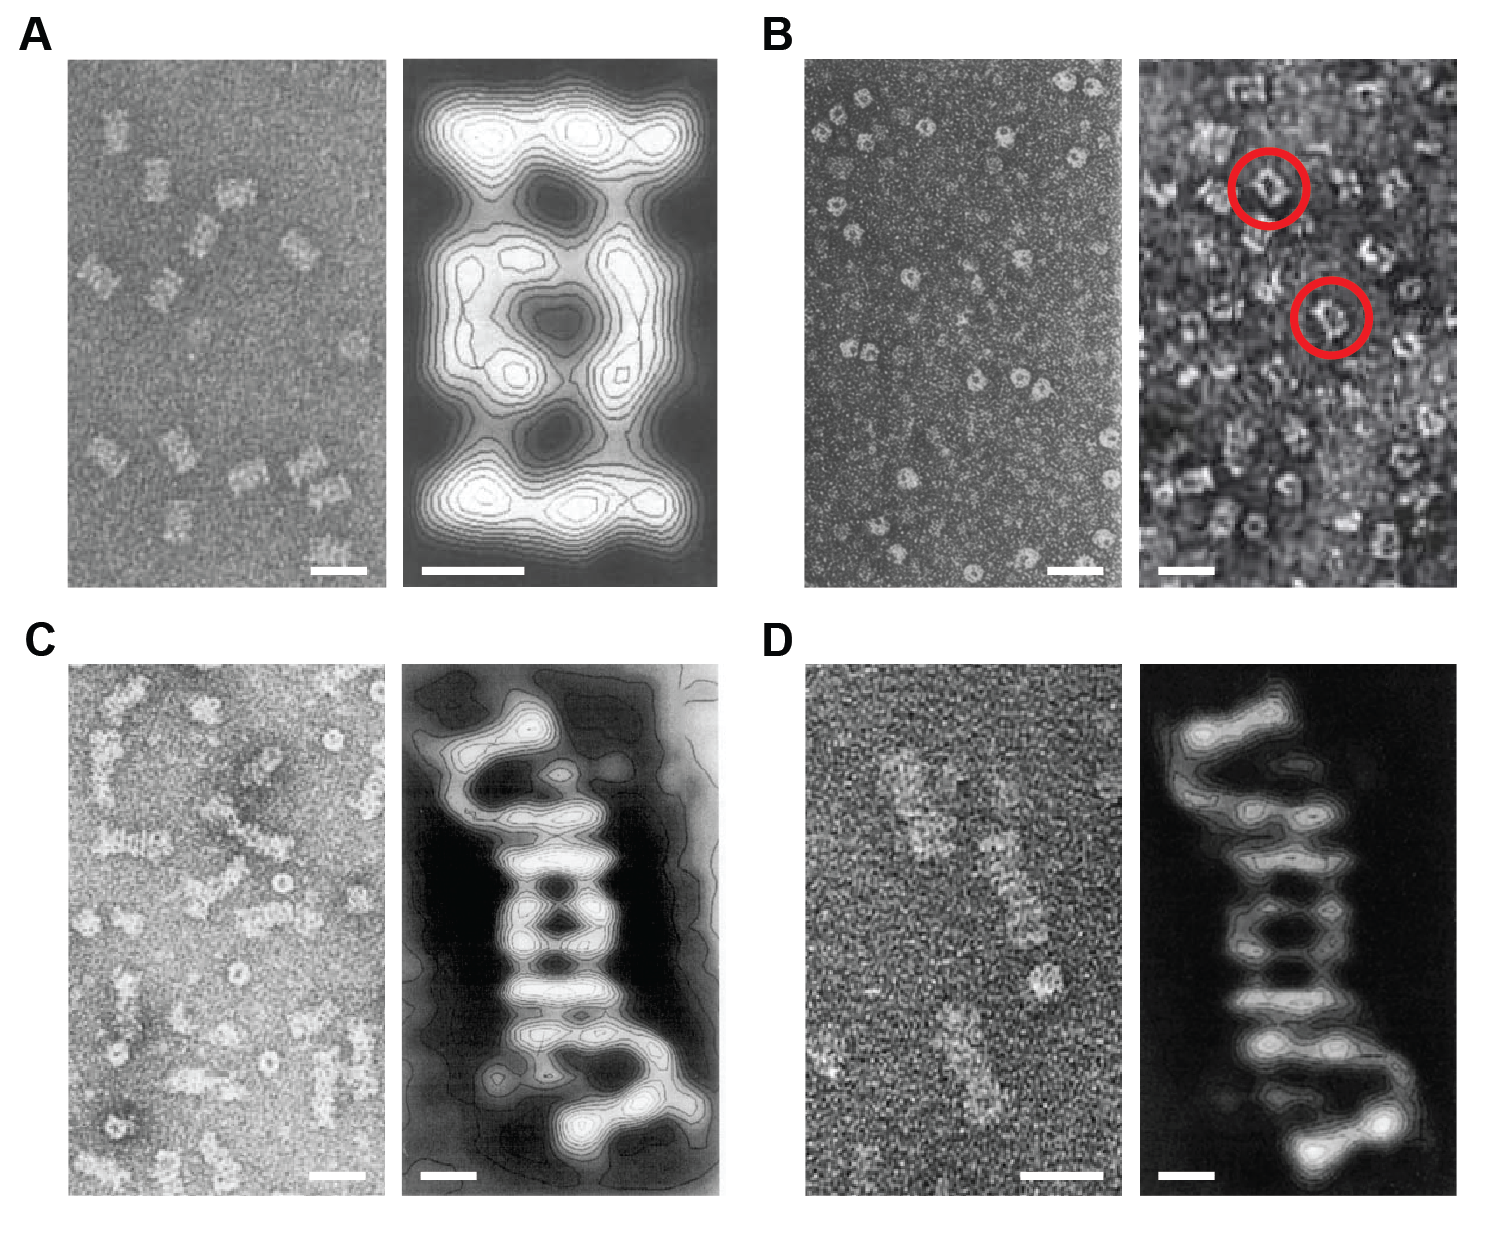
\includegraphics[width=\columnwidth]{intro/figure2.png}
	\mycaption{Electron microscopy images of the 20S and 26S proteasomes from mammals and plants}{
		\textbf{(A)} Images of 20S proteasomes purified from rat skeletal muscle.  On the left is an electron micrograph of the 20S particles negatively stained with sodium phosphotungstate, while on the right is a close-up image with overlaid contour plots generated by correlation averaging of approximately 300 individual images negatively stained with ammonium molybdate.  \textbf{(B)} Images of the first 20S proteasomes purified from different plant species.  On the left are proteasomes isolated from tobacco leaves, while on the right are proteasomes from potato tubers, both negatively stained with uranyl acetate.  The typical barrel-shaped structures are indicated with red circles.  \textbf{(C)} Images of 26S proteasomes purified from rat liver.  On the left is an electron micrograph of the 26S particles negatively stained with uranyl acetate, while on the right is a close-up image with overlaid contour plots generated by correlation averaging of 215 individual images.  \textbf{(D)} Images of 26S proteasomes purified from spinach leaves.  On the left is an electron micrograph of the 26S particles negatively stained with uranyl acetate, while on the right is a close-up image with overlaid contour plots generated by correlation averaging of 450 individual images.  In all cases, scale bars represent 25 nm for the electron micrograph images and 5 nm for close-up images generated by averaging.  The images were modified from references \citep{baumeister88, fujinami94, kremp86, schliephacke91, yoshimura93}.
	}
	\label{fig:proteasomeelec}
\end{figure}
	  Purification of the 20S fraction from HeLa cells followed by SDS-PAGE also gave rise to this stereotypical protein banding pattern and shape \citep{schmid84}, and this was followed shortly thereafter by the first description of plant prosomes, purified from tobacco leaf extracts using similar sedimentation protocols in ATP-free buffers \citep{kremp86}.  In these later cases, the purified preparations had strong peptidase activity but little to no RNase activity, thus leading to the conclusion that the CP is actually a protease.  Once its true function in protein turnover was confirmed, the moniker for the particle was changed to `proteasome' \citep{arrigo88}.  
	Subsequently, the 20S particle was purified from other plant tissues, including dry pea seeds, potato tubers, mung bean seedlings, and leaves from both spinach and wheat \citep{murray97, ozaki92, schliephacke91, skoda92}.  These purifications were typically performed using sequential anion exchange and size-exclusion chromatography steps in the absence of ATP, hence only the CP was isolated.  Their remarkable similarity in protein composition and structure, as observed by SDS-PAGE and electron microscopy, respectively, coupled with the fact that several of the plant subunits cross-reacted with antibodies against their yeast, human, rat and Xenopus counterparts, strongly implied that the CP was conserved and widely distributed among eukaryotes \citep{schliephacke91}.
	The complete 26S proteasome (i.e. the CP capped at one or both ends by the RP) was subsequently discovered by the purification of ubiquitin conjugate-degrading activity from rabbit reticulocytes \citep{hough86}.  While it had been well established that major catabolic processes in animal cells involved the ATP-dependent proteolysis of selective substrates \citep{etlinger77}, the enzyme(s) responsible for this activity had yet to be identified.  Taking advantage of the new ability to synthesize ubiquitylated substrates such as 125I-labelled ubiquitin-lysozyme conjugates \citep{hough86-1xVPf}, a protocol was developed to purify the responsible ATP-dependent protease.  Through a series of anion exchange and size exclusion chromatography steps followed by glycerol gradient sedimentation, all of which were performed in ATP-containing buffers, the responsible activity was isolated \citep{hough86, hough87}. The active enzyme turned out to be the 20S proteasome (i.e. the CP) along with a number of additional polypeptides which together formed a 26S particle, thus providing the first direct link between ubiquitylation and a protease \citep{ganoth88, hough87, waxman87}.  SDS-PAGE analysis of these preparations identified a host of new polypeptides in the 35-100 kDa range in addition to the known CP subunits, which were later shown to comprise a second stable complex, the RP.  Shortly thereafter, the RP was demonstrated to have ATPase activities attributable to the RPT subunits, which help in substrate unfolding and maintaining CP-RP association \citep{armon90}.  Electron microscopic images of the full 26S particle then revealed its diagnostic quaternary structure in which the CP is capped by one or two RPs which sit over the axial pores for substrate entry (Figure \ref{fig:proteasomeelec} C; \citep{peters91, yoshimura93}).
	The existence of a similar 26S proteasome in plants was initially implied by the detection of an ATP-dependent activity in oat and wheat germ extracts capable of degrading ubiquitylated proteins \citep{hatfield89, vierstra88}.  This was followed some years later by the first isolation of a complete plant 26S proteasome holocomplex from spinach leaves \citep{fujinami94}.  As with the mammalian forms, purification was achieved by anion exchange and size exclusion chromatography, followed by glycerol gradient centrifugation, all in the presence of ATP to stabilize the CP-RP association.  These spinach preparations were, like their rabbit reticulocyte counterparts, able to rapidly degrade ubiquitylated substrates in an ATP-dependent manner, and further analysis by native-PAGE, SDS-PAGE and electron microscopy revealed the complete subunit composition and ``caterpillar-like'' structure of the plant particle (Figure \ref{fig:proteasomeelec} D; \citep{fujinami94}).  Similar purifications were successful using rice suspension culture cells and garlic cloves \citep{malik04, yanagawa99}, which were accompanied by the first demonstrations that proteasome inhibitors designed for their mammalian counterparts were effective with the plant particles, suggesting very similar enzymatic mechanisms \citep{ozaki92, woffenden98}.
	Despite its prevalence as a genetic model, purification of the 26S proteasome from the flowering plant \textit{Arabidopsis thaliana} was not reported until several years after other plant species \citep{yang04}.  First protocols involved differential PEG precipitation followed by anion exchange and size exclusion chromatography, with the latter exploiting the large size of the holoprotease.  More recently, an improved one-step affinity method was developed \citep{book10}, based on the strategies that had been successfully employed in yeast \citep{leggett05}.  Here, epitope-tagged proteasomes were generated by genetically replacing the subunit PAG1 with a variant bearing a C-terminal FLAG tag; this tagged particle could then be purified with appropriate affinity matrices and released in its native condition with FLAG peptide.  This approach enables rapid and robust purification of the whole 26S proteasome complex when performed in the presence of ATP, or enables purification of the CP sub-particle when performed in the absence of ATP \citep{book10}. This affinity method has considerable advantages compared to previous conventional chromatographic approaches \citep{yang04} as it is both faster and more reliable, produces higher yields per gram of tissue (~6 µg/g). 
\begin{figure}[p]
	\centering
	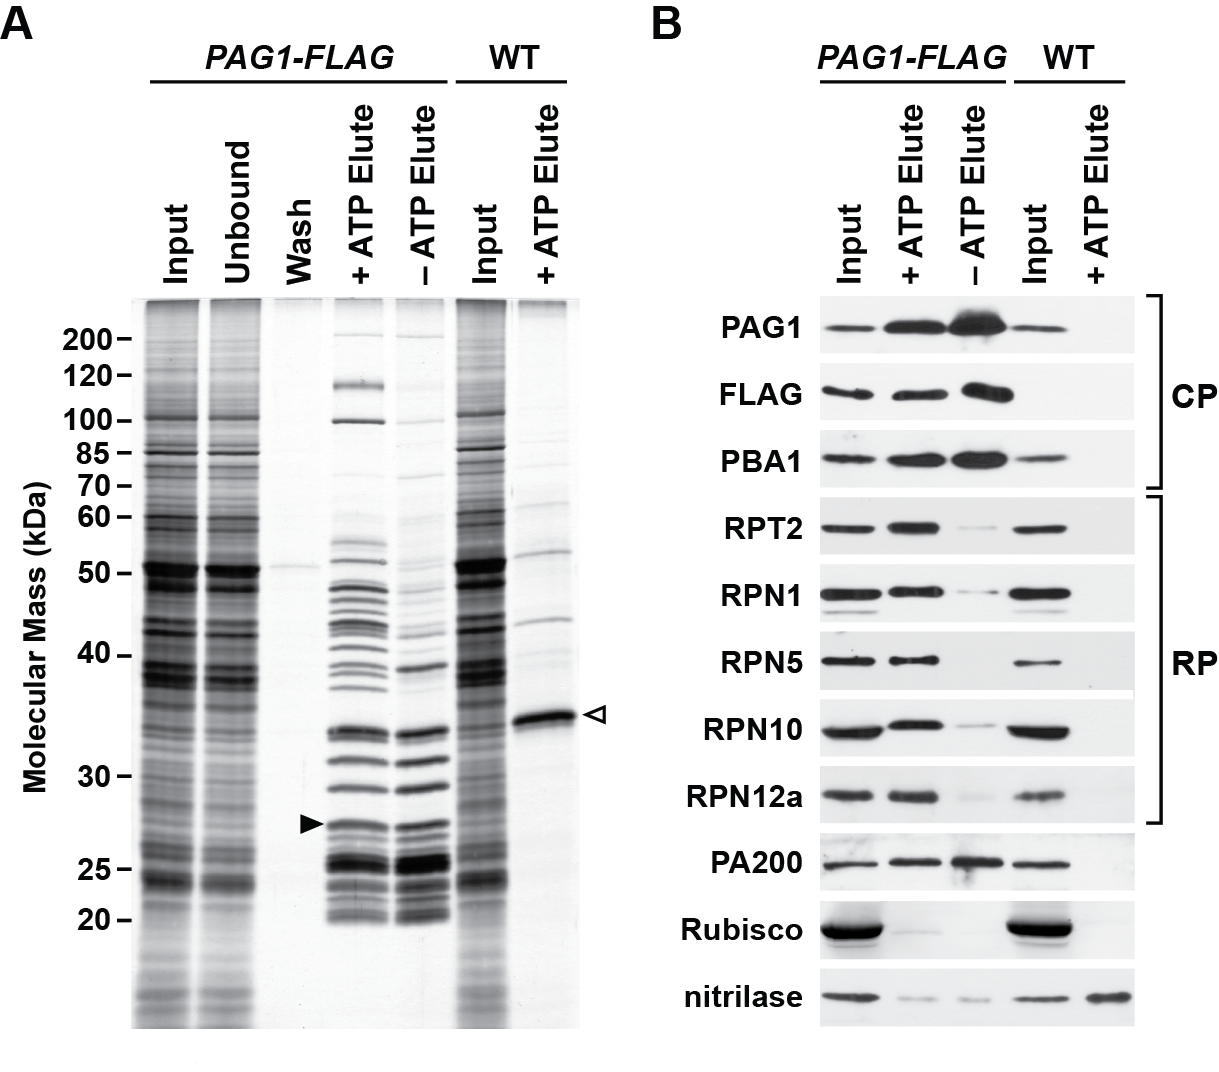
\includegraphics[width=\columnwidth]{intro/pag1affinity.png}
	\mycaption{Affinity purification of 26S proteasomes from \textit{pag1-1 PAG1-FLAG} plants}{
		\textbf{(A)} SDS-PAGE analysis of the affinity purification steps.  Total protein extracts from 10 day old wild-type (WT) and \textit{pag1-1 PAG1-FLAG} plants were incubated with anti-FLAG affinity resin, washed, and competitively eluted with the FLAG peptide.  The procedure was performed in the presence or absence of ATP, and the input, unbound, washed and eluted fractions were subjected to SDS-PAGE and the gel stained for protein with silver.  The black arrowhead indicates the PAG1-FLAG protein, while the open arrowhead identifies nitrilase, which is non-specifically enriched during the purification.  \textbf{(B)} Immunoblot detection of various 26S proteasome subunits in the affinity-purified preparations shown in A. Subunits tested include the CP subunits PAG1 and PBA1, the RP subunits RPT2, RPN1, RPN5, RPN10 and RPN12a, and the alternate capping particle PA200.  Other proteins tested include the Rubisco small subunit and nitrilase.  This figure was modified from reference \citep{book10}.
	}
	\label{fig:pag1affinity}
\end{figure}
This milder more rapid technique also prevents breakdown of some subunits, in particular RPN10, which is sensitive to post-homogenization proteolysis \citep{yang04}.  One caveat is that the epitope tag, given its exposed position and flexible structure, might be sensitive to proteolytic cleavage following tissue homogenization.  For the PAG1-FLAG protocol, chymostatin was found to effectively block the interfering protease \citep{book10}.  An example of such preparations analyzed by SDS-PAGE followed by immunoblotting with antibodies against several proteasome subunits, are shown in Figures  \ref{fig:pag1affinity} A and B, respectively.


\section{26S Proteasome Substrate Processing}
	A variety of proteins help the 26S proteasome process ubiquitylated substrates. Some include key constituents of the complex itself such as RPN11, which is a metalloprotease that uses a zinc-coordinated active site to release the ubiquitin moieties isopeptide-linked to substrates \citep{verma02, worden14}.  Through RPN11 and other loosely associated deubiquitylating enzymes such as UBP6/USP14 \citep{hanna06, sakata11}, bound ubiquitins are actively recycled.
	Substrate selection by the 26S proteasome is dictated by several ubiquitin receptors intrinsic to the RP lid, including RPN10, RPN13 (in yeast), and DSS1/SEM1 \citep{fatimababy10, finley09, lin11, paraskevopoulos14, sakata12, van96}, and possibly RPN1 in the base \citep{elsasser02}.  RPN10 binds ubiquitin via defined ubiquitin-interacting motifs (UIMs), of which yeast, human and \textit{Arabidopsis} RPN10 contain 1, 2 and 3 in tandem, respectively \citep{fatimababy10, finley09, fu98, lin11, van96}.  By contrast, RPN13 binds ubiquitin via a pleckstrin-like receptor for ubiquitin (PRU) domain, which is structurally distinct from UIMs but binds to the same hydrophobic patch on ubiquitin \citep{husnjak08, schreiner08}.  More recently, DSS1/SEM1 was also found to be a proteasomal ubiquitin receptor \citep{paraskevopoulos14}.  It had previously resisted identification due to both its small size, which prevented visualization by standard protein stains following sodium dodecyl sulfate-polyacrylamide gel electrophoresis (SDS-PAGE), and its paucity of lysine and arginine residues, which complicated detection by conventional mass spectrometric methods.  Only with the use of top-down mass spectrometry of 26S proteasome complexes was DSS1/SEM1 first detected in intact 26S proteasomes from \textit{Arabidopsis} \citep{russell13}.  
	In addition to these core ubiquitin receptors, there are several extra-proteasomal ubiquitin-binding proteins that shuttle ubiquitylated cargo to the RP.  They work by virtue of ubiquitin-associated (UBA) domains that bind ubiquitin, combined with a ubiquitin-like (UBL) domain that interacts with the intrinsic ubiquitin receptors such as RPN10.  Important shuttle factors in plants include RAD23, DSK2, and DDI1 \citep{farmer10, fatimababy10, finley09, lin11}, though many other ubiquitin-binding proteins are known in other species \citep{husnjak12}.  Numerous other factors also associate sub-stoichiometrically with the mature CP and RP sub-complexes, including deubiquitylating enzymes, several E3 ligases and protein kinases, and a collection of protein folding chaperones \citep{besche14, book10, leggett02, xie00}.


\section{Proteasome Isotypes}
	Genetic Analysis of CP and RP subunits shows lethality etc


\section{Proteasome Inhibition and Proteasome Degredation}


\section{26S Proteasome Assembly}
	Not surprisingly given its intricate architecture, construction of the 26S proteasome requires a large collection of assembly factors that work in synchrony.  Included are chaperones required for the correctly ordered assembly of the $\alpha$- and $\beta$-rings of the CP and the RPT ring of the RP, which in yeast involve the Pba1/2 and Pba3/4 heterodimers for the CP \citep{kusmierczyk08, le07, tomko13}, and Nas2, Nas6, Hsm3 and Rpn14 for the RP \citep{funakoshi09, roelofs09, saeki09, tomko13}.  Additional chaperones then mediate assembly of the final particle.  UMP1 is required to connect the two $\alpha$/$\beta$ half-barrels to generate the complete CP.  Once its job is finished UMP1 is degraded, thus becoming the first proteolytic substrate of the fully assembled CP \citep{ramos98}.  ECM29 stabilizes the association of assembled CP and RP and provides a final quality control checkpoint for mature 26S proteasomes \citep{besche14, lehmann10}.  Finally, in some situations, the RP is replaced entirely by alternate capping particles such as PA200 (also known as Blm10) or CDC48 \citep{barthelme12, book10, schmidt05}.  The functions of these caps are not yet clear, but recent proposals for PA200 have it participating in 26S proteasome assembly, helping shuttle proteasomes into the nucleus, and/or generating a ubiquitin-independent proteasome containing CP and PA200 only \citep{dange11, sadre-bazzaz10, weberruss13}.


\section{Proteasome Associated Proteins (PAPs)}
Beyond those associated proteins already mentioned that are involved in substrate processing and assembly, there are a variety of proteins that are known to interact with the yeast and mammalian proteasomes. These include: loosely associated DUBS such as UCH37, and etc etc


\section{Conclusions}

The \textit{Arabidopsis} 26S proteasome exists in planta as a diverse array of complexes containing multiple subunit isoforms and interacting proteins \citep{book10, fu99, yang04}.  To facilitate biochemical analysis of the plant particle, we developed a rapid and robust affinity purification protocol that enables isolation of intact 26S proteasomes, and the individual CP and RP (Chapter 3) sub-complexes, by genetically replacing individual subunits with FLAG-tagged versions \citep{book10}.  Such a strategy was based on a similar approach used successfully with yeast, where the proteasome subunits Pre1, Rpt1 and Rpn11 were appended with either FLAG or Protein A tags to permit effective affinity enrichment \citep{leggett05}.  Using the recently described structures of the 26S proteasome \citep{bhattacharyya14, lander12, lasker12}, we identified subunits in the CP (PAG1) and as demonstrated in this thesis RP (RPT4) which had solvent exposed N- or C-termini that were potentially appropriate for appending the epitope tag (see Figures \ref{fig:proteasomefunc} B and C).  


\begin{singlespace}
\bibliographystyle{plant_cell_final}
\renewcommand\bibname{Literature Cited}
\bibliography{UPS}
\end{singlespace}


